\documentclass[12pt,a4paper,landscape]{article}
\usepackage{mathtools,graphicx,url,xparse}
\title{My First \LaTeX{} Document}
\author{Scott Harvey-Whittle\thanks {The Open University Student}}
\date{February 2024}
\graphicspath{images/}
\begin{document}
\maketitle
\begin{flushleft}
    

\section{\textbf{Bold},\textit{Italics}, \underline{underlines}, and \emph{emph}}
Some of the \textbf{greatest}

Greatest above is now \textbf{bold} 

discoveries in \underline{science} 

Science Above is now \underline{Underlined}

were made by \textbf{\textit{accident}}.

Accident above is now in \textit{Italics}


Some of the greatest \emph{discoveries} in science 
were made by accident.

Notice how the "emph" function above turns the word discoveries into  \emph{Italics.}

\textit{Some of the greatest \emph{discoveries} 
in science were made by accident.}

In this Example notice that we set the sentance to write in \textit{italics}, but when we use the "emph" function it turns the Italics off. 

\textbf{Some of the greatest \emph{discoveries} 
in science were made by accident.}

Same with this example. We use the \textbf{bold} function for the whole sentence but when we use the emph function it makes the word \textit{discoveries} in Italics.

\section{Creating lists in \LaTeX{}}

\subsection{Unordered Lists(Bullet Points)}

In order for you to use unordered lists you need to use the backslash begin Itemise function.

\begin{itemize}
  \item The individual entries are indicated with a black dot, a so-called bullet.
  \item The text in the entries may be of any length.
\end{itemize}
Remember that if we are beginning something we need to end it. So we need to use the backslash end itemise function. 

\subsection{Ordered lists}

\begin{enumerate}
\item The labels consists of sequential numbers.
\item The numbers starts at 1 with every call to the enumerate environment.
\item remember to use begin and end enumerate to create this sort of list. 
\end{enumerate}

\subsection{Nested Lists}

\begin{enumerate}
 \item The labels consists of sequential numbers.
 \begin{itemize}
 \item The individual entries are indicated with a black dot, a so-called bullet.
 \item The text in the entries may be of any length.
 \end{itemize}
 \item The numbers starts at 1 with every call to the enumerate environment.
 \item How this list works: 
 \begin{itemize}
 \item A Nested list is a combination of Ordered and Unordered lists. 
 \item You start with Enumerate, then Item (no curly brackets)Write your numbered statement. Then you begin itemise 
 Then item. Enter your statement. Then end Itemise and lastly end .
 \end{itemize}
\end{enumerate}
Notice that the words \textbf{enumerate} and \textbf{itemise} and in curly brackets but there is nothing after the word \textbf{item}.

\section{Math}
\subsection{Inline Math writing}
To use the inline math tool we use the Dollar sign at the beginning and the end of our math. example:

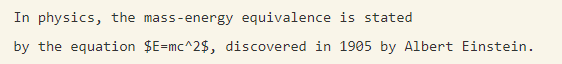
\includegraphics{Inline Math Example.PNG}



Notice that the output of this looks as follows:

In physics, the mass-energy equivalence is stated 
by the equation $E=mc^2$, discovered in 1905 by Albert Einstein.

There are Various ways ti use inline math mode. The first is the Dollar sign, you can backslash start math (the word math in curly brackets) and then backslash end math. 
\subsection{Display Math Mode}

The mass-energy equivalence is described by the famous equation
\[ E=mc^2 \] discovered in 1905 by Albert Einstein. 

Notice in this section, whe formula is diplayed for presentation. we do this as follows:

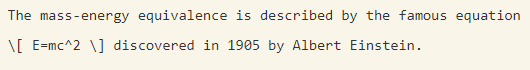
\includegraphics{Display Math Mode Example.PNG}

You can also start and end your math with 2 dollar signs. 

\section{Other Math bits and bobs}
Subscripts in math mode are written as $a_b$ and superscripts are written as $a^b$. These can be combined and nested to write expressions such as

\[ T^{i_1 i_2 \dots i_p}_{j_1 j_2 \dots j_q} = T(x^{i_1},\dots,x^{i_p},e_{j_1},\dots,e_{j_q}) \]
 
We write integrals using $\int$ and fractions using $\frac{a}{b}$. Limits are placed on integrals using superscripts and subscripts:

\[ \int_0^1 \frac{dx}{e^x} =  \frac{e-1}{e} \]

Lower case Greek letters are written as $\omega$ $\delta$ etc. while upper case Greek letters are written as $\Omega$ $\Delta$.

Mathematical operators are prefixed with a backslash as $\sin(\beta)$, $\cos(\alpha)$, $\log(x)$ etc.

The above was written as follows:

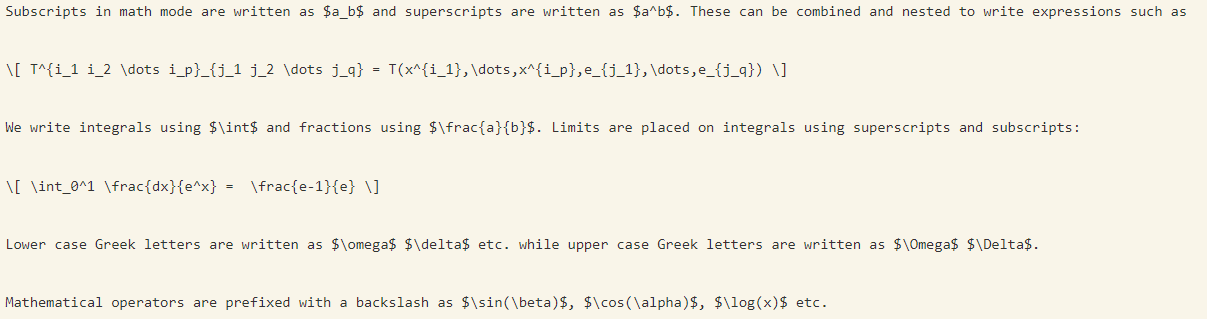
\includegraphics[scale=0.4]{Math Example Bits and Bobs.PNG} 
 



\section{Basic Math Functions}
Here is a Few Examples of Basic Math Functions

\subsection{Add, Minus, Divide and Times}
\begin{enumerate}
    \item $$4+4=8$$
    \item $$8-4=4$$
    \item $$20\div4=5$$
    \item $$10\times10=100$$
\end{enumerate}
\subsection{Sub and Super Script}

Subscript uses underscores while superscript uses the arrow pointing up. This arrow is normally found above the number 6 on your keyboard. 

\begin{enumerate}
    \item $2^4$ $6^9$ $8^3$ (Superscript)
    \item $4_5$ $8_4$ $8_1$ (Subscript)
\end{enumerate}
\subsection{Square Root}
You can get a Square root by typing backslash then sqrt then open curly brackets followed by Number then closed curly brackets. 
$$\sqrt{36}$$
\subsection{Pie}
To Enter Pie you enter backslash pi 
Here is an example

$$\pi$$
\end{flushleft}
\end{document}
